\documentclass[11pt]{article}

% review mode = anonymous + line numbers (for ARR submission).
% Switch to "final" for camera-ready, "preprint" for non-anonymous arXiv.
\usepackage[review]{acl}

\usepackage{times}
\usepackage{latexsym}
\usepackage[T1]{fontenc}
\usepackage[utf8]{inputenc}
\usepackage{microtype}
\usepackage{inconsolata}

\usepackage{amsmath}
\usepackage{amssymb}
\usepackage{booktabs}
\usepackage{multirow}
\usepackage{graphicx}
\usepackage{pgfplots}
\pgfplotsset{compat=1.18}
\usepackage{tikz}
\usepackage{xcolor}

\title{Norm-Bounded Federated Updates against\\ Language-Guided Gradient Inversion Attacks}

% Authors anonymized for review.
\author{Anonymous Submission \\ ARR Cycle May 2026}

\begin{document}
\maketitle

\begin{abstract}
Vision-language models (VLMs) enable a new class of gradient inversion attacks in federated learning, where a malicious server uses natural-language queries to reconstruct private client data with semantic targeting~\citep{geminio2024}. We make two findings about this threat. First, adversarially robust VLMs designed to defend against input perturbations~\citep{fare2024,simclip2024,tecoa2023} do not provide privacy protection: they raise Geminio's gradient-amplification loss ratio by 57--61\% on medical data, and on UAV imagery three of six robust variants increase mean end-to-end attack F1 above vanilla CLIP (3-seed multi-run). Robustness in this sense is not a substitute for gradient-channel defense. Second, a simple per-update DP mechanism we call \emph{Norm-Bounded Federated Updates} (NBFU)---L2 clipping of the entire client update plus calibrated Gaussian noise---substantially reduces attack success and generalizes across three reconstruction algorithms (HF-GradInv, IG, GradInversion). On UAV imagery NBFU at $\varepsilon{=}5$ drives mean attack F1 to $\le 0.13$ across all three attacks (vs.\ $\le 0.33$ clean); on medical imagery it cuts mean F1 by 50--56\% (from 0.67 to 0.29--0.33). Defense on medical leaves a non-trivial residual, and the headline budget ($\varepsilon{=}5$) destabilizes single-step classifier training, so the defense is best deployed at suspect FL rounds rather than throughout training. A $\sigma{=}0$ ablation shows that clipping and noise contribute via different mechanisms: clipping disrupts scale-sensitive image-prior regularizers (TV, BatchNorm statistics), while noise breaks scale-invariant cosine-similarity matching. Removing either component leaves at least one attack family largely undefended. We release configs and code for the four attack methods, the defense, and the reproducible multi-seed sweep.
\end{abstract}


\section{Introduction}

Federated learning (FL) promises privacy by replacing data sharing with gradient sharing~\citep{fedavg2017}. Gradient inversion attacks (GIAs) undermine that promise by recovering private inputs from shared gradients~\citep{dlg2019,ig2020,gradinversion2021}. A recent line of work~\citep{robbing2022,fishing2023,geminio2024} extends GIAs to active malicious servers that craft global model parameters to amplify target gradients before reconstruction.

\citet{geminio2024} introduce a \emph{language-guided} variant in which the server provides a natural-language description of valuable data (e.g., \textit{``any chest X-ray showing pneumonia''}) and a pretrained vision-language model (VLM)~\citep{clip2021} is used to reshape the malicious model's loss surface so that gradients become dominated by query-matching samples. The result is a targeted attack with a flexible, semantically meaningful interface. Because the attacker's discrimination ability scales with VLM quality, this class of attack is expected to strengthen as VLMs improve.

We study this threat from a defense standpoint and report two findings. The first is \emph{negative}: adversarially robust VLMs---a defense category designed to harden CLIP against input perturbations~\citep{tecoa2023,fare2024,simclip2024}---do not defend against language-guided gradient inversion and in fact strengthen it on medical imagery by 57--61\% (Section~\ref{sec:vlm}). The second is \emph{positive}: calibrated differentially private FL with per-update gradient clipping~\citep{dpsgd2016}, which we refer to as Norm-Bounded Federated Updates (NBFU), reduces attack F1 to near zero on UAV imagery and substantially on medical imagery (Section~\ref{sec:nbfu}). The defense generalizes across the three competitive reconstruction algorithms we test (HF-GradInv, IG, GradInversion); a fourth (DLG) is too weak at our image scale to inform defense evaluation (Section~\ref{sec:generalize}).

We further give an analytical argument (Section~\ref{sec:method}) for why clipping is sufficient: it normalizes the gradient norm to a fixed bound $C$ independent of the attacker's loss-ratio amplification, so the post-defense signal-to-noise ratio depends only on $C$, the calibrated noise scale, and the model dimension---not on how strongly the attacker amplified the target. Measurements of pre-clip gradient norms (15.6 on medical, 527.0 on UAV) match this prediction.

\paragraph{Contributions.}
\begin{enumerate}
\itemsep0pt
    \item A negative result for VLM-side defense: adversarial robustness in CLIP variants strengthens, rather than mitigates, language-guided gradient inversion.
    \item A positive result for gradient-side defense: NBFU at $\varepsilon{=}5$ (sensitivity-$2C$ calibration; see Section~\ref{sec:method}) drives mean attack F1 to $\le 0.13$ on UAV across the three reconstruction algorithms we test, and reduces medical F1 by 50--56\% on average (3-seed multi-run validation).
    \item A mechanistic decomposition via $\sigma{=}0$ ablation: clipping defends attacks with scale-sensitive priors; noise defends scale-invariant cosine matching. Both components are required for attack-agnostic defense.
    \item Utility curves under NBFU on the underlying classification task, characterizing the privacy--utility frontier at multiple $\varepsilon$.
    \item A reproducible benchmark covering four GIAs (HF-GradInv, IG, GradInversion, DLG), three batch sizes, and three random seeds.
\end{enumerate}


\section{Background and Threat Model}
\label{sec:background}

\subsection{Federated learning}
We consider FedSGD~\citep{fedavg2017}: at each round $t$ the server distributes parameters $\theta_t$; client $i$ samples a private batch $B_t^i$ of size $n$ and shares the averaged gradient
\[
G_t^i = \frac{1}{n} \sum_{(x,y) \in B_t^i} \nabla_{\theta_t} \mathcal{L}\big(F_{\theta_t}(x);\, y\big).
\]

\subsection{Gradient inversion}
Optimization-based GIAs~\citep{dlg2019,ig2020,gradinversion2021} reconstruct $B_t^i$ by solving
\begin{equation}
\bar{B}^* = \arg\min_{\bar{B}}\; \delta\!\left(G_t^i,\; G(\bar{B}; \theta_t)\right) + \mathcal{R}(\bar{B}),
\label{eq:gia}
\end{equation}
where $\delta$ is a gradient-matching distance (typically Euclidean or cosine) and $\mathcal{R}$ is an image prior (e.g., total variation or feature-space regularization).

\subsection{Geminio: language-guided malicious models}
\citet{geminio2024} consider an active server that crafts $\theta_Q$ such that, for any client batch, samples matching a natural-language query $Q$ have per-sample loss $\mathcal{L}_{\text{target}}$ amplified by a factor $R$ relative to non-matching samples:
\[
\mathcal{L}\big(F_{\theta_Q}(x_{\text{target}})\big) \;\approx\; R \cdot \mathcal{L}\big(F_{\theta_Q}(x_{\text{other}})\big).
\]
Because per-sample gradient magnitude scales with loss, the averaged client gradient becomes dominated by the target subset, enabling reconstruction via Equation~\ref{eq:gia} on a effectively single-sample signal even when $n$ is moderately large.

\subsection{Threat model}
Following~\citet{geminio2024,fishing2023}, we consider an active server that may modify $\theta_t$ but not the architecture. The server holds a pretrained VLM and an unlabeled auxiliary image set, and observes the client's $G_t^i$. Notably, the VLM operates on \emph{clean} server-side images, not on adversarial perturbations of client inputs---this distinction motivates our negative result on adversarially robust VLMs (Section~\ref{sec:vlm}).


\section{Defense: Norm-Bounded Federated Updates}
\label{sec:method}

\subsection{Definition}
Before sharing $G$, the client applies two operations:
\begin{align}
G_{\text{clip}} &= G \cdot \min\!\left(1,\; \frac{C}{\|G\|_2}\right), \label{eq:clip}\\
G_{\text{def}} &= G_{\text{clip}} + \mathcal{N}(0, \sigma^2 I), \label{eq:noise}
\end{align}
with $\sigma = 2C \cdot \sqrt{2 \ln(1.25/\delta)} / \varepsilon$ following the analytic Gaussian mechanism~\citep{gaussianmechanism2018}. We refer to this composite operation as \emph{Norm-Bounded Federated Updates} (NBFU).

\paragraph{Privacy semantics.}
NBFU performs \emph{per-update} clipping (the entire averaged client update) rather than \emph{per-example} clipping (each per-sample gradient before averaging). We make the DP guarantee precise.

\emph{Adjacency.} Datasets $B, B'$ are neighboring if one record in the client's batch has been substituted: $|B \triangle B'| = 2$ with $|B| = |B'| = n$.

\emph{Mechanism.} Let $f(B) = \mathrm{clip}_C\!\big((1/n)\sum_{(x,y)\in B} \nabla_\theta \mathcal{L}(F_\theta(x); y)\big)$ where $\mathrm{clip}_C(v) = v \cdot \min(1, C/\|v\|_2)$. NBFU releases $\tilde f(B) = f(B) + \mathcal{N}(0, \sigma^2 I)$.

\emph{Sensitivity.} For any neighboring $B, B'$, $\|f(B) - f(B')\|_2 \le 2C$ because $\|f(B)\|_2, \|f(B')\|_2 \le C$ by construction. The bound is tight in the worst case (two clipped vectors on antipodal points of the radius-$C$ ball).

\emph{Guarantee.} With $\sigma = 2C\sqrt{2 \ln(1.25/\delta)} / \varepsilon$, the analytic Gaussian mechanism~\citep{gaussianmechanism2018} gives $(\varepsilon, \delta)$-DP for $\tilde f$ under the above adjacency, per single FL round. Over $T$ rounds, advanced composition or a moments accountant gives the cumulative budget; with i.i.d.\ noise across rounds and the analytic mechanism this is roughly $\varepsilon_T \approx \varepsilon\sqrt{2T\ln(1/\delta')} + T\varepsilon(e^\varepsilon - 1)$ for small $\varepsilon$, $\delta' \gg \delta$.

\emph{Comparison with record-level DP-SGD.} Record-level DP-SGD~\citep{dpsgd2016} clips per-example gradients to $C$ before averaging, so the per-record sensitivity scales as $C/n$ and the noise can be calibrated to that. NBFU's per-update bound (sensitivity $2C$) is therefore looser by a factor of $\Theta(n)$ at the same $\varepsilon$. Our motivation for the per-update notion is operational: many FL deployments share only averaged updates, the active malicious-model threat targets recovery within a single round (where per-example clipping is the client's choice, not the server's), and the per-update mechanism requires no changes to existing FL aggregation. We do not claim NBFU is a substitute for record-level DP-SGD when stronger guarantees are needed; it is a deployable defense matched to the Geminio threat model.

\subsection{Analytical argument: SNR after defense}
\label{sec:snr}
Two scopes are relevant. The \emph{optimizer} updates only the 148K-parameter classifier head; the ResNet-18 backbone weights are not modified during training. The \emph{shared update} that the attacker observes, however, is the gradient of the loss with respect to every parameter that has \texttt{requires\_grad=True}---the full $d\approx 1.13{\times}10^{7}$ parameter set, since we leave the backbone unfrozen even though it is not optimized (76\% of the gradient $\ell_2$ norm is in the backbone, see Section~\ref{sec:nbfu-mechanism}). Inversion attacks search the full $d$-dimensional space, so the relevant $d$ for both the noise norm and the SNR bound is the larger one. The expected $\ell_2$ norm of the noise term in Equation~\ref{eq:noise} is $\|\mathcal{N}\| \approx \sigma\sqrt{d}$. After clipping, the signal norm satisfies $\|G_{\text{clip}}\|_2 \le C$ regardless of $\|G\|$. Hence the post-defense signal-to-noise ratio satisfies
\begin{equation}
\mathrm{SNR} \;\le\; \frac{C}{\sigma\sqrt{d}}.
\label{eq:snr}
\end{equation}
This bound is independent of the attacker's amplification factor $R$. As Geminio's loss ratio grows, the unclipped $\|G\|$ grows, but clipping renormalizes the signal to scale $C$ and the calibrated noise is set to $C$ as well, so $R$ drops out.

\paragraph{Two complementary defense components.}
Equation~\ref{eq:snr} captures the noise side of the argument: small SNR is sufficient. Clipping plays a separate role, which Equation~\ref{eq:snr} alone does not show: it bounds sensitivity (enabling the DP analysis above) and it disrupts reconstruction objectives whose value depends on \emph{absolute} gradient magnitude---specifically Euclidean matching and image-prior regularizers (TV, BatchNorm-statistic) that are scale-sensitive. Pure cosine-similarity matching is scale-invariant, so against such attacks the noise does the entire defense work. Section~\ref{sec:nbfu-mechanism} dissects which component is doing what, attack by attack, via a $\sigma{=}0$ ablation.

\paragraph{Numerical SNR.}
For our setup ($C{=}1$, $\varepsilon{=}5$, $\delta{=}10^{-5}$), $\sigma \approx 1.94$ (using sensitivity $2C$) and Equation~\ref{eq:snr} gives $\mathrm{SNR} \approx 1.5{\times}10^{-4}$: the defended gradient is dominated by noise. Empirical gradient norms (Table~\ref{tab:gradnorms}) confirm the regime.


\section{Experimental Setup}
\label{sec:setup}

\paragraph{Datasets and tasks.}
We test on two image classification benchmarks: \textbf{ChestMNIST}~\citep{medmnistv2} (15-way, $28{\times}28$ chest X-rays upsampled to $224{\times}224$) and \textbf{UAVScenes}~\citep{uavscenes2024} (18-way, $224{\times}224$ aerial drone imagery).

\paragraph{Model.}
A ResNet-18~\citep{resnet2016} backbone (ImageNet-pretrained) with a 3-layer classifier head (512$\to$256$\to$64$\to N$ classes). The optimizer updates only the classifier head (148K parameters), but the backbone keeps \texttt{requires\_grad=True} so gradients propagate through it; the \emph{shared} update consequently spans the full $d \approx 1.13{\times}10^{7}$ parameters and the attacker uses them all (76\% of $\|G\|^2$ resides in the backbone). Our main experiments use \texttt{model.eval()} for the victim forward/backward (BatchNorm uses fixed running statistics), following the convention in~\citet{breaching2023}. Recent systematizations note that this configuration can simplify inversion relative to a realistic training-mode client. We therefore include a BN \texttt{train}-mode subset (Section~\ref{sec:bntrain}) and find that, while train mode lowers the clean attack on medical (0.500 vs.\ 0.667 in eval), the NBFU defense margin is actually larger in train mode.

\paragraph{VLMs.}
Vanilla CLIP ViT-L/14~\citep{clip2021}, BiomedCLIP~\citep{biomedclip2023}, and adversarially robust variants SimCLIP-2/4~\citep{simclip2024}, FARE-2/4~\citep{fare2024}, and TeCoA-2/4~\citep{tecoa2023}. The numeric suffix denotes the adversarial training budget ($\epsilon = k/255$).

\paragraph{Reconstruction algorithms.}
We use four optimization-based GIAs from~\citet{breaching2023}: HF-GradInv~\citep{hfgradinv2024} (Geminio's default), IG~\citep{ig2020}, GradInversion~\citep{gradinversion2021,deepinversion2020}, and DLG~\citep{dlg2019,idlg2020}. All run for 24{,}000 iterations with seed-controlled random initialization.

\paragraph{Defense.}
NBFU as defined in Equations~\ref{eq:clip}--\ref{eq:noise}, with clipping norm $C{=}1.0$, $\delta{=}10^{-5}$, batch size $n{=}8$ unless stated otherwise. We sweep $\varepsilon \in \{0.1, 1, 5, 10, 50\}$.

\paragraph{Metrics.}
\textbf{Attack F1} at cosine threshold 0.90 between reconstruction and target output-layer gradients (the metric used in~\citet{geminio2024}); \textbf{LPIPS}~\citep{lpips2018}, lower is better; and PSNR. We report mean $\pm$ standard deviation over three seeds (42, 123, 256). All comparisons in tables are at the same seed unless aggregated.


\section{Robust VLMs Do Not Help Defense}
\label{sec:vlm}

\subsection{Two metrics, different stories}
For each VLM, we train Geminio's malicious model on five medical queries and six UAV queries~\citep{geminio2024} and evaluate the attack using two metrics. The \emph{loss ratio}---average per-sample loss on the top-10\% query-matching auxiliary images divided by average loss on the bottom 90\%---measures Geminio's gradient amplification during the malicious-model training phase (the metric used by~\citet{geminio2024}). The end-to-end \emph{attack F1} (Section~\ref{sec:setup}) measures reconstruction success against a victim batch using HF-GradInv. They can disagree, and on our two domains they do.

\begin{figure}[t]
\centering
% Loss ratio across VLM variants on medical and UAV.
% Higher = stronger attack.
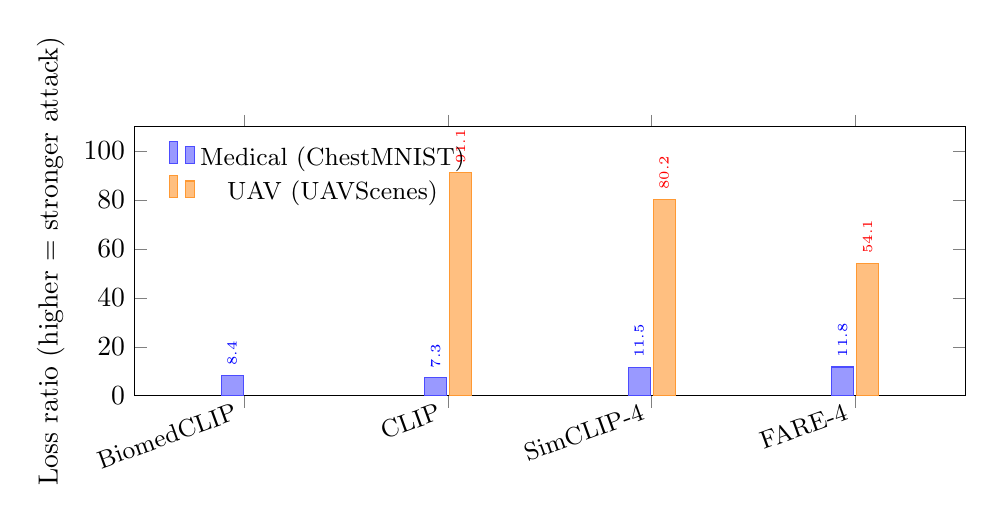
\begin{tikzpicture}
\begin{axis}[
    width=\columnwidth,
    height=5cm,
    ybar=1pt,
    bar width=8pt,
    enlarge x limits=0.18,
    ylabel={Loss ratio (higher = stronger attack)},
    symbolic x coords={BiomedCLIP, CLIP, SimCLIP-4, FARE-4},
    xtick=data,
    xticklabel style={font=\small, rotate=20, anchor=east},
    ytick={0,20,40,60,80,100},
    ymin=0, ymax=110,
    legend pos=north west,
    legend style={font=\small, draw=none, fill=none},
    nodes near coords={\pgfmathprintnumber[fixed,precision=1]{\pgfplotspointmeta}},
    nodes near coords style={font=\tiny, rotate=90, anchor=west},
    every node near coord/.append style={
        /pgf/number format/assume math mode=true
    },
]
\addplot+[fill=blue!40, draw=blue!70, /pgf/nan/.style={hide point=true}] coordinates {
    (BiomedCLIP, 8.39)
    (CLIP, 7.32)
    (SimCLIP-4, 11.46)
    (FARE-4, 11.75)
};
\addplot+[fill=orange!50, draw=orange!80] coordinates {
    (CLIP, 91.12)
    (SimCLIP-4, 80.20)
    (FARE-4, 54.11)
};
\legend{Medical (ChestMNIST), UAV (UAVScenes)}
\end{axis}
\end{tikzpicture}

\caption{Average per-domain Geminio loss ratio across VLM variants. Higher = stronger gradient amplification on query-matching auxiliary samples. On medical imagery, adversarially robust VLMs (SimCLIP-4, FARE-4) \emph{increase} amplification by 57--61\% over vanilla CLIP.}
\label{fig:vlm}
\end{figure}

\subsection{Loss-ratio: robust VLMs amplify more on medical}
Figure~\ref{fig:vlm} summarizes the average loss ratio per (domain, VLM) pair. On medical imagery, both robust VLMs increase the loss ratio over vanilla CLIP: SimCLIP-4 by 57\%, FARE-4 by 61\%. BiomedCLIP, a domain-specialized but non-robust encoder, also gives a modest 15\% increase. On UAV imagery, vanilla CLIP already achieves a 91$\times$ loss ratio; robust VLMs do not improve it and FARE-4 reduces it by 41\%. The amplification effect is consistent with the intuition that robust encoders learn more semantically meaningful features---useful for distinguishing chest X-ray pathologies that look alike to a non-specialized model.

\subsection{End-to-end attack F1: the picture flips by domain}
\label{sec:vlm-endtoend}
Loss ratio measures the malicious model's \emph{targeting ability}; it does not by itself imply higher reconstruction success. Table~\ref{tab:vlm_endtoend} reports HF-GradInv attack F1 on each VLM-trained malicious model with no defense.

\begin{table}[h]
\centering
\small
\begin{tabular}{lcc}
\toprule
VLM & Medical F1 & UAV F1 \\
\midrule
Vanilla CLIP   & \textbf{0.750$\pm$.13} & 0.250$\pm$.13 \\
SimCLIP-2 & 0.250$\pm$.00 & 0.375$\pm$.13 \\
SimCLIP-4 & 0.542$\pm$.19 & 0.250$\pm$.00 \\
FARE-2    & 0.625$\pm$.13 & 0.417$\pm$.19 \\
FARE-4    & 0.375$\pm$.13 & 0.292$\pm$.19 \\
TeCoA-2   & 0.333$\pm$.19 & 0.250$\pm$.00 \\
TeCoA-4   & 0.542$\pm$.07 & \textbf{0.458$\pm$.07} \\
\bottomrule
\end{tabular}
\caption{End-to-end attack F1 (HF-GradInv, no defense), mean$\pm$std over 3 seeds (42, 123, 256), using malicious models trained with each VLM. On medical, vanilla CLIP gives the strongest attack and every robust variant has lower mean F1 (gap 0.13--0.50). On UAV, three robust variants (SimCLIP-2, FARE-2, TeCoA-4) yield higher mean F1 than vanilla CLIP, though the gap (0.13--0.21) is closer to the seed-to-seed variance.}
\label{tab:vlm_endtoend}
\end{table}

The pattern is \emph{domain-dependent}. On medical, vanilla CLIP yields mean F1 = 0.750 (over 3 seeds) and every robust variant has lower mean (0.25--0.625); robust VLMs \emph{weaken} the end-to-end attack despite raising loss ratio, and the gap is well outside seed variance for at least SimCLIP-2 (0.250$\pm$.00), FARE-4 (0.375$\pm$.13), and TeCoA-2 (0.333$\pm$.19). On UAV, the relationship inverts: vanilla CLIP gives mean F1 = 0.250 and the strongest robust variant (TeCoA-4) gives 0.458; three of six robust variants (SimCLIP-2, FARE-2, TeCoA-4) sit above vanilla CLIP, though the gap (0.13--0.21) is close to the seed-to-seed variance. We interpret this as follows. Geminio's loss ratio measures how sharply the malicious model concentrates gradient energy on a target sample; this targeting is one ingredient of attack success. End-to-end F1 also depends on whether the targeted gradient \emph{pattern} is invertible, which interacts with the encoder's feature geometry. In visually similar domains (chest X-rays), vanilla CLIP's coarse features happen to produce a more directly invertible target pattern despite weaker targeting. In visually distinctive domains (aerial imagery), robust encoders' sharper features tend to produce both stronger targeting \emph{and} more invertible patterns, though the effect is modest.

\paragraph{Perceptual metrics agree on medical, are flat on UAV.}
LPIPS (lower is better) and PSNR (higher is better) corroborate the medical-domain story. Vanilla CLIP on medical gives mean LPIPS = 0.93 / PSNR = 11.18; every robust variant gives lower LPIPS (0.55--0.69) and higher PSNR (11.76--14.35), with TeCoA-4 the most perceptually accurate reconstruction (LPIPS 0.554, PSNR 14.35). The gap between F1 (gradient-cosine threshold) and LPIPS is informative: robust VLMs produce reconstructions that look more like the targets visually, but whose output-layer gradients do not match as sharply at the F1 threshold. On UAV the LPIPS spread is modest (CLIP 0.70 vs.\ robust 0.60--0.72) and matches the small F1 gap.

\subsection{Implication}
The original \emph{a priori} hope---that adversarially robust VLMs would protect against language-guided gradient inversion---fails on both metrics: they at best leave the attack unchanged, and on UAV they actively help the attacker. The mechanism is a threat-model mismatch (SimCLIP/FARE/TeCoA defend against \emph{adversarial inputs}, but Geminio uses the VLM on \emph{clean} server-side images). VLM-side robustness is therefore not a substitute for gradient-channel defense. The remainder of the paper studies that defense.


\section{Norm-Bounded Federated Updates Reduce the Attack}
\label{sec:nbfu}

\subsection{Privacy-budget sweep}
Figure~\ref{fig:eps} shows attack F1 and average per-sample gradient cosine similarity as a function of $\varepsilon$ for HF-GradInv on the canonical Geminio queries (sensitivity-$2C$ calibration (Section~\ref{sec:method})). NBFU defends across the full range $\varepsilon \in [0.1, 50]$. On UAV, F1 stays at 0 for every $\varepsilon$ tested. On medical, F1 sits in 0.25--0.50 across the range; while it fluctuates non-monotonically (the threshold metric is sensitive to single-sample crossings at $n{=}8$), the continuous $\overline{\cos}$ stays in 0.35--0.56 (vs.\ 0.92 at clean), confirming that the underlying gradient signal is consistently degraded.

\begin{figure}[t]
\centering
% Attack F1 and avg cosine similarity vs NBFU epsilon (HF-GradInv, 2C calibration).
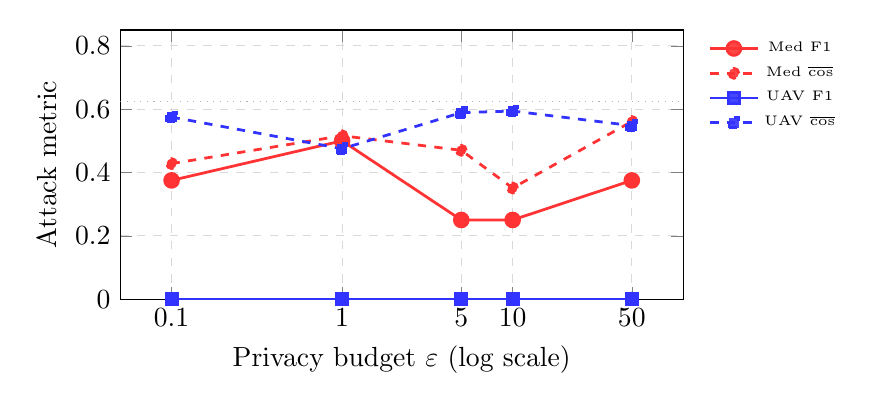
\begin{tikzpicture}
\begin{axis}[
    width=0.72\columnwidth,
    height=5cm,
    xlabel={Privacy budget $\varepsilon$ (log scale)},
    ylabel={Attack metric},
    xmode=log,
    log basis x=10,
    xmin=0.05, xmax=100,
    ymin=0, ymax=0.85,
    grid=major,
    grid style={dashed, gray!30},
    legend pos=outer north east,
    legend style={font=\tiny, draw=none, fill=white, fill opacity=0.9, text opacity=1},
    mark size=2.5pt,
    every axis plot/.append style={line width=1pt},
    xtick={0.1,1,5,10,50},
    xticklabels={0.1, 1, 5, 10, 50},
]
\addplot[color=red!80, mark=*] coordinates {
    (0.1, 0.375)
    (1.0, 0.500)
    (5.0, 0.250)
    (10.0, 0.250)
    (50.0, 0.375)
};
\addlegendentry{Med F1}
\addplot[color=red!80, mark=*, dashed, mark size=1.8pt] coordinates {
    (0.1, 0.428)
    (1.0, 0.516)
    (5.0, 0.470)
    (10.0, 0.351)
    (50.0, 0.561)
};
\addlegendentry{Med $\overline{\cos}$}
\addplot[color=blue!80, mark=square*, mark size=2pt] coordinates {
    (0.1, 0.000)
    (1.0, 0.000)
    (5.0, 0.000)
    (10.0, 0.000)
    (50.0, 0.000)
};
\addlegendentry{UAV F1}
\addplot[color=blue!80, mark=square*, mark size=1.8pt, dashed] coordinates {
    (0.1, 0.575)
    (1.0, 0.475)
    (5.0, 0.589)
    (10.0, 0.594)
    (50.0, 0.548)
};
\addlegendentry{UAV $\overline{\cos}$}

\draw[dotted, gray!60] (axis cs:0.05,0.625) -- (axis cs:100,0.625);
\end{axis}
\end{tikzpicture}

\caption{Attack F1 (solid) and average sample-level gradient cosine similarity $\overline{\cos}$ (dashed) vs.\ NBFU privacy budget $\varepsilon$ (HF-GradInv, batch size 8, seed 42, sensitivity $2C$). UAV F1 is 0 across the range; medical F1 is non-monotonic but $\overline{\cos}$ stays well below the no-defense value of 0.92.}
\label{fig:eps}
\end{figure}

\subsection{Mechanism: which component is doing what}
\label{sec:nbfu-mechanism}
Empirical pre-clip gradient norms set the scale at which clipping operates:
\begin{table}[h]
\centering
\small
\begin{tabular}{lcc}
\toprule
Domain & $\|G\|$ before clip & $C/\|G\|$ \\
\midrule
Medical & 15.6 & 0.064 \\
UAV & 527.0 & 0.0019 \\
\bottomrule
\end{tabular}
\caption{Pre-clip gradient norms (HF-GradInv, $C{=}1$). Geminio's amplification is much larger on UAV (loss ratio $\sim$91$\times$) than on medical ($\sim$8$\times$); clipping removes most of that amplification.}
\label{tab:gradnorms}
\end{table}

\paragraph{Decomposing the defense via $\sigma{=}0$.}
To separate clipping from noise, we run a clipping-only condition (apply Equation~\ref{eq:clip} but skip Equation~\ref{eq:noise}). Table~\ref{tab:cliponly} compares clean F1, $\sigma{=}0$ clipping-only F1, and full NBFU at $\varepsilon{=}5$.

\begin{table}[h]
\centering
\small
\begin{tabular}{llccc}
\toprule
Domain & Attack & Clean & Clip-only & NBFU $\varepsilon{=}5$ \\
\midrule
\multirow{3}{*}{Med.}
 & HF-GradInv     & 0.667$\pm$.07 & 0.625$\pm$.00 & 0.292$\pm$.07 \\
 & IG             & 0.667$\pm$.07 & 0.583$\pm$.19 & 0.292$\pm$.07 \\
 & GradInv        & 0.667$\pm$.07 & 0.500$\pm$.00 & 0.333$\pm$.14 \\
\midrule
\multirow{3}{*}{UAV}
 & HF-GradInv     & 0.250$\pm$.13 & 0.125$\pm$.13 & 0.125$\pm$.22 \\
 & IG             & 0.208$\pm$.07 & 0.208$\pm$.07 & 0.042$\pm$.07 \\
 & GradInv        & 0.333$\pm$.14 & 0.125$\pm$.13 & 0.000$\pm$.00 \\
\bottomrule
\end{tabular}
\caption{Clipping-only ($\sigma{=}0$) vs.\ full NBFU ($\varepsilon{=}5$), mean$\pm$std over 3 seeds (42, 123, 256). Clipping handles attacks with scale-sensitive image priors (IG and GradInversion on medical drop by 13--25\% under clipping alone); noise handles scale-invariant cosine matching (UAV IG sees \emph{zero} effect from clipping but full defense once noise is added).}
\label{tab:cliponly}
\end{table}

The decomposition reveals two regimes. \emph{First}, on UAV with IG (pure cosine matching with TV), clipping alone has zero mean effect (0.208 clean, 0.208 clip-only); the cosine-similarity reconstruction objective is scale-invariant, so dividing the gradient by a scalar does not change the optimization landscape. The defense in this regime comes entirely from noise (0.208 $\to$ 0.042). \emph{Second}, for medical IG and GradInversion---both of which use scale-sensitive image priors---clipping alone provides 13--25\% of the F1 reduction, because shrinking the gradient changes the relative weighting between the gradient-matching loss and the prior. Adding noise on top closes the remaining gap.

\paragraph{Implication.} The often-cited intuition that ``clipping bounds sensitivity, noise provides DP'' is correct but incomplete. In the GIA setting both components also contribute \emph{empirically} via different mechanisms: clipping disrupts scale-sensitive reconstruction priors, noise breaks gradient-matching at the SNR level. Removing either component leaves at least one attack family largely undefended.

\subsection{Comparison with other defenses}
Table~\ref{tab:defenses} compares NBFU with the standard defenses tested in~\citet{geminio2024} and with VLM-side robust encoders. Only NBFU provides reliable defense with formal $(\varepsilon,\delta)$-DP guarantees.

\begin{table}[t]
\centering
\small
\begin{tabular}{lccc}
\toprule
Defense & Med.\ F1 & UAV F1 & Reliable \\
\midrule
None (FedSGD)        & 0.667 & 0.250 & --- \\
Pruning 99\%         & inconsist. & inconsist. & no \\
Laplace noise        & inconsist. & inconsist. & no \\
SimCLIP-4            & 0.542 & 0.250 & no \\
FARE-4               & 0.375 & 0.292 & no \\
FedAvg 5 epochs      & 0.000 & 0.375 & partial \\
FedAvg 20 epochs     & 0.000 & 0.250 & partial \\
\textbf{NBFU} $\varepsilon{=}5$ (2C)  & \textbf{0.292} & \textbf{0.125} & \textbf{yes} \\
\textbf{NBFU} $\varepsilon{=}10$ (2C) & \textbf{0.250}$^\dagger$ & \textbf{0.000}$^\dagger$ & \textbf{yes} \\
\bottomrule
\end{tabular}
\caption{Defense comparison against Geminio (HF-GradInv) on canonical queries. ``None'' through SimCLIP-4/FARE-4 and the NBFU $\varepsilon{=}5$ row are mean F1 over 3 seeds; FedAvg and NBFU $\varepsilon{=}10$ rows ($^\dagger$) are single-seed (seed 42). Although SimCLIP-4 and FARE-4 reduce mean F1 on medical, they raise the underlying loss-ratio amplification by 57--61\% (Section~\ref{sec:vlm}) and do not lower UAV F1 below the no-defense baseline, so we judge them unreliable as defenses. NBFU is the only reliable defense with formal $(\varepsilon,\delta)$-DP guarantees (sensitivity $2C$ calibration). Continuous $\overline{\cos}$ at NBFU $\varepsilon{=}5$ is 0.47 (medical) and 0.59 (UAV), vs.\ 0.92 / 0.88 clean.}
\label{tab:defenses}
\end{table}


\section{Defense Generalizes Across Reconstruction Algorithms}
\label{sec:generalize}

We rerun the $\varepsilon{=}5$ defense against three additional reconstruction algorithms: IG~\citep{ig2020} (cosine matching with total-variation prior), GradInversion~\citep{gradinversion2021} (Euclidean matching with TV, norm, and BatchNorm-statistic priors), and DLG~\citep{dlg2019} (Euclidean matching, no prior). We also include the original HF-GradInv~\citep{hfgradinv2024} for comparison. Three seeds (42, 123, 256), 24{,}000 iterations.

\subsection{Multi-seed results}
Table~\ref{tab:multiseed} reports mean $\pm$ standard deviation. Figure~\ref{fig:multiseed} visualizes the same data. Across all six (attack, domain) combinations with non-trivial clean baselines, NBFU $\varepsilon{=}5$ reduces F1, with the defense effect substantially exceeding the seed-to-seed variance.

\begin{table}[t]
\centering
\small
\begin{tabular}{llcc}
\toprule
Domain & Attack & Clean F1 & NBFU $\varepsilon{=}5$ F1 \\
\midrule
\multirow{3}{*}{Medical}
 & HF-GradInv     & 0.667$\pm$.07 & 0.292$\pm$.07 \\
 & IG             & 0.667$\pm$.07 & 0.292$\pm$.07 \\
 & GradInversion  & 0.667$\pm$.07 & 0.333$\pm$.14 \\
\midrule
\multirow{3}{*}{UAV}
 & HF-GradInv     & 0.250$\pm$.13 & 0.125$\pm$.22 \\
 & IG             & 0.208$\pm$.07 & 0.042$\pm$.07 \\
 & GradInversion  & 0.333$\pm$.14 & 0.000$\pm$.00 \\
\bottomrule
\end{tabular}
\caption{Multi-seed defense generalization at the sensitivity-$2C$ calibration (Section~\ref{sec:method}) (3 seeds, 24k iterations). NBFU at $\varepsilon{=}5$ reduces attack F1 across all six (domain, attack) cells. UAV is fully or near-fully defended; medical defense is partial but consistent across attacks (mean drop 50--56\%).}
\label{tab:multiseed}
\end{table}

\begin{figure}[t]
\centering
% Multi-seed defense effectiveness across attacks at 2C calibration (3 seeds).
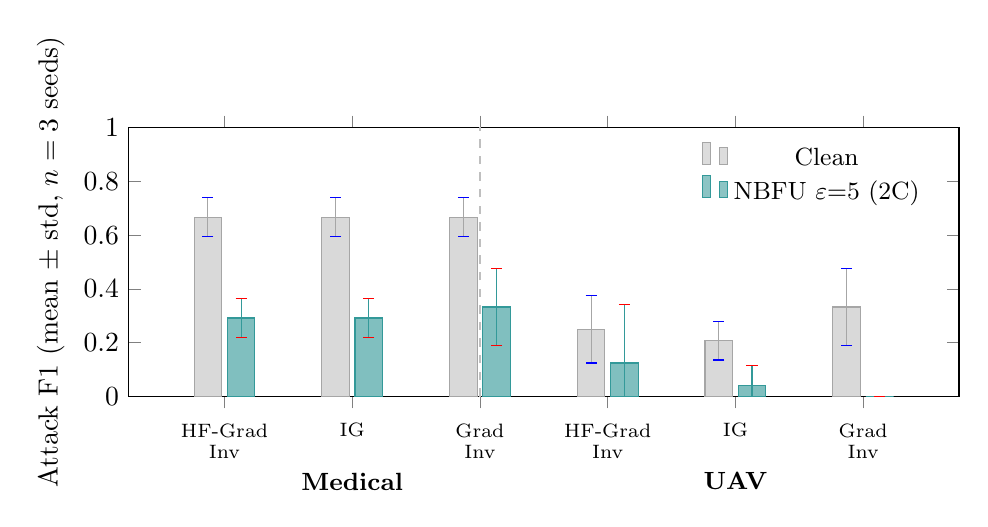
\begin{tikzpicture}
\begin{axis}[
    width=\columnwidth,
    height=5cm,
    ybar=2pt,
    bar width=10pt,
    enlarge x limits=0.15,
    ylabel={Attack F1 (mean $\pm$ std, $n=3$ seeds)},
    symbolic x coords={HF-GradInv, IG, GradInv, HF-GradInv*, IG*, GradInv*},
    xtick={HF-GradInv, IG, GradInv, HF-GradInv*, IG*, GradInv*},
    xticklabels={\shortstack{HF-Grad\\Inv}, IG, \shortstack{Grad\\Inv}, \shortstack{HF-Grad\\Inv}, IG, \shortstack{Grad\\Inv}},
    xticklabel style={font=\scriptsize, align=center, yshift=-2pt},
    extra x ticks={IG, IG*},
    extra x tick labels={Medical, UAV},
    extra x tick style={
        major tick length=0pt,
        xticklabel style={yshift=-22pt, font=\small\bfseries}
    },
    ymin=0, ymax=1.0,
    legend pos=north east,
    legend style={font=\small, draw=none, fill=white, fill opacity=0.9, text opacity=1},
    error bars/y dir=both,
    error bars/y explicit,
]
\addplot+[fill=gray!30, draw=gray!70] coordinates {
    (HF-GradInv, 0.667) +- (0,0.072)
    (IG, 0.667) +- (0,0.072)
    (GradInv, 0.667) +- (0,0.072)
    (HF-GradInv*, 0.250) +- (0,0.125)
    (IG*, 0.208) +- (0,0.072)
    (GradInv*, 0.333) +- (0,0.144)
};
\addlegendentry{Clean}

\addplot+[fill=teal!50, draw=teal!80] coordinates {
    (HF-GradInv, 0.292) +- (0,0.072)
    (IG, 0.292) +- (0,0.072)
    (GradInv, 0.333) +- (0,0.144)
    (HF-GradInv*, 0.125) +- (0,0.217)
    (IG*, 0.042) +- (0,0.072)
    (GradInv*, 0.000) +- (0,0.000)
};
\addlegendentry{NBFU $\varepsilon{=}5$ (2C)}

\draw[gray!50, dashed] (axis cs:GradInv,0) -- (axis cs:GradInv,1.0);
\end{axis}
\end{tikzpicture}

\caption{Defense generalization across three reconstruction algorithms (HF-GradInv, IG, GradInversion). Bars show mean attack F1 over three seeds, error bars show standard deviation. NBFU $\varepsilon{=}5$ reduces F1 in all six (domain, attack) cells.}
\label{fig:multiseed}
\end{figure}

\subsection{Algorithm-dependent residuals}
On medical, mean F1 reductions are 56\%, 56\%, and 50\% for HF-GradInv, IG, and GradInversion respectively---essentially identical across attacks. On UAV, the defense drops F1 by 50--100\% (full defense for GradInversion); the UAV HF-GradInv cell has high seed variance (std $0.22$, with one seed at $0.375$ where clean was also $0.375$). The remaining residual on medical reflects three factors: (i) Geminio's medical loss-ratio amplification is moderate ($\sim$8$\times$) so the unclipped gradient norm is small to begin with, leaving less for clipping to remove; (ii) image-prior regularizers (TV, BatchNorm-statistic matching) provide candidate-side signal that is independent of the gradient channel and partially compensates for noisy gradients; (iii) the F1 metric at $n{=}8$ has high variance, as discussed in Section~\ref{sec:nbfu-mechanism} (Table~\ref{tab:cliponly}).

\subsection{Sensitivity to the clipping bound $C$}
\label{sec:csens}
We sweep $C \in \{0.1, 0.5, 1.0, 2.0, 5.0\}$ at fixed $\varepsilon{=}5$ (HF-GradInv, seed 42).

\begin{table}[h]
\centering
\small
\begin{tabular}{lcccc}
\toprule
$C$ & Med F1 & Med $\overline{\cos}$ & UAV F1 & UAV $\overline{\cos}$ \\
\midrule
0.1 & 0.250 & 0.355 & 0.125 & 0.659 \\
0.5 & 0.375 & 0.475 & 0.125 & 0.711 \\
1.0 & 0.250 & 0.343 & 0.000 & 0.625 \\
2.0 & 0.500 & 0.574 & 0.125 & 0.680 \\
5.0 & 0.125 & 0.338 & 0.000 & 0.563 \\
\bottomrule
\end{tabular}
\caption{Attack F1 vs.\ clipping bound $C$ at fixed $\varepsilon{=}5$. The medical F1 row is U-shaped because noise scales with $C$ ($\sigma = 2C\sqrt{2\ln(1.25/\delta)}/\varepsilon$): at small $C$ defense comes from tight clipping; at large $C$ defense comes from large noise; an intermediate $C$ (around 2) is the weakest defense regime. UAV defense is near-saturated across the range.}
\label{tab:csens}
\end{table}

Two practical takeaways. \emph{First}, the defender does \emph{not} have a single optimal $C$ at fixed $\varepsilon$; both very tight $C$ ($\lesssim 0.5$) and very loose $C$ ($\gtrsim 5$) defend medical to F1 $\le 0.25$, while $C{=}2$ leaves F1 = 0.5. \emph{Second}, an adaptive $C$ procedure (e.g., setting $C$ to a low percentile of observed per-update gradient norms) would naturally avoid the weakest-defense regime. We leave full adaptive-$C$ implementation, in the style of~\citet{dpsfl2024}, to future work.

\subsection{Realism check: BatchNorm train mode}
\label{sec:bntrain}
The main experiments use \texttt{model.eval()} (BN uses running statistics). Several recent works flag that \texttt{train}-mode BN (where each forward pass updates running averages and uses batch statistics) substantially complicates inversion. We rerun HF-GradInv on both domains with the victim in \texttt{train} mode (and the breaching framework's convention of setting \texttt{momentum=None} to allow recovery), at $\varepsilon{=}5$ NBFU vs.\ clean, seed 42.

\begin{table}[h]
\centering
\small
\begin{tabular}{llccc}
\toprule
Domain & BN mode & Clean & NBFU $\varepsilon{=}5$ & Drop \\
\midrule
\multirow{2}{*}{Med.}
 & eval (multi-seed) & 0.667 & 0.292 & 56\% \\
 & train (seed 42)   & 0.500 & 0.125 & 75\% \\
\midrule
\multirow{2}{*}{UAV}
 & eval (multi-seed) & 0.250 & 0.125 & 50\% \\
 & train (seed 42)   & 0.250 & 0.000 & 100\% \\
\bottomrule
\end{tabular}
\caption{BN train mode vs.\ eval mode (HF-GradInv, $\varepsilon{=}5$, sensitivity $2C$). Train mode lowers the clean attack on medical (0.667 $\to$ 0.500) but the NBFU defense margin is \emph{larger} in train mode in both domains. UAV clean is unchanged.}
\label{tab:bntrain}
\end{table}

Train mode reduces the clean attack F1 on medical (consistent with the systematization claims), but the defense margin is preserved and actually larger: medical NBFU drops to F1=0.125 in train mode (vs.\ 0.292 in eval), and UAV reaches F1=0 in train mode under NBFU. The qualitative conclusions of the paper---that NBFU substantially reduces attack F1, with a larger margin on UAV than on medical---hold in both BN regimes. Multi-seed train-mode evaluation is left to future work.

\subsection{Batch-size effect}
Figure~\ref{fig:batch} shows attack F1 versus batch size $n \in \{8, 16, 32\}$ for HF-GradInv at the sensitivity-$2C$ calibration (the only attack that fits in GPU memory at $n \ge 16$). The relative defense margin shrinks with larger batches on medical: a 50\% reduction at $n{=}8$ collapses to 7\% at $n{=}32$. This follows from two interacting factors: averaging over more samples shrinks the unclipped gradient norm $\|G\|$, so the clipping factor $C/\|G\|$ is closer to one (less aggressive clipping); and Geminio's per-target gradient signal is diluted by more non-target samples, raising the clean-baseline F1 ceiling (0.75 $\to$ 0.91 from B8 to B32). On UAV, F1 stays at or near 0 under NBFU across all three batch sizes. Practical takeaway: $C$ should be tuned to the expected per-update gradient norm at the deployment batch size, and $\varepsilon$ may need to be tightened for large-batch deployments to maintain the same defense level.

\begin{figure}[t]
\centering
% Attack F1 vs batch size at 2C calibration (HF-GradInv, seed 42).
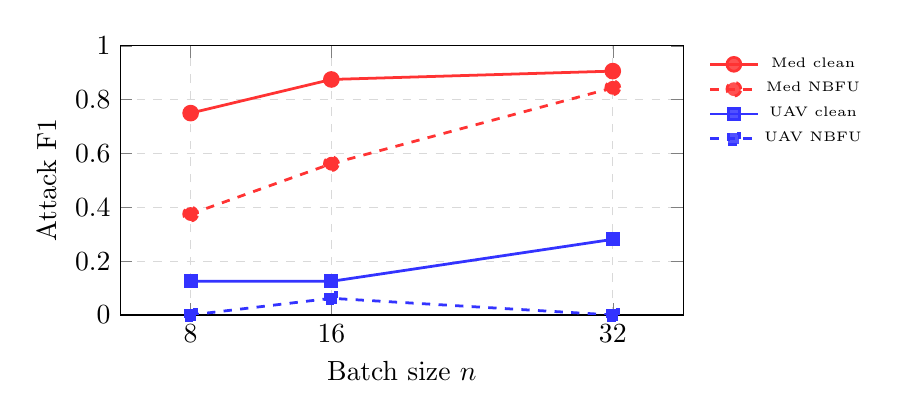
\begin{tikzpicture}
\begin{axis}[
    width=0.72\columnwidth,
    height=5cm,
    xlabel={Batch size $n$},
    ylabel={Attack F1},
    xtick={8,16,32},
    xmin=4, xmax=36,
    ymin=0, ymax=1.0,
    grid=major,
    grid style={dashed, gray!30},
    legend pos=outer north east,
    legend style={font=\tiny, draw=none, fill=white, fill opacity=0.85, text opacity=1},
    mark size=2.5pt,
    every axis plot/.append style={line width=1pt},
]
\addplot[color=red!80, mark=*] coordinates {
    (8, 0.750)
    (16, 0.875)
    (32, 0.906)
};
\addlegendentry{Med clean}

\addplot[color=red!80, mark=*, dashed] coordinates {
    (8, 0.375)
    (16, 0.562)
    (32, 0.844)
};
\addlegendentry{Med NBFU}

\addplot[color=blue!80, mark=square*, mark size=2pt] coordinates {
    (8, 0.125)
    (16, 0.125)
    (32, 0.281)
};
\addlegendentry{UAV clean}

\addplot[color=blue!80, mark=square*, mark size=2pt, dashed] coordinates {
    (8, 0.000)
    (16, 0.062)
    (32, 0.000)
};
\addlegendentry{UAV NBFU}
\end{axis}
\end{tikzpicture}

\caption{Attack F1 vs.\ batch size for HF-GradInv at NBFU $\varepsilon{=}5$ ($2C$ calibration). Defense margin narrows at larger batches as the unclipped gradient norm decreases and the clean-baseline F1 ceiling rises.}
\label{fig:batch}
\end{figure}


\section{Privacy--Utility Trade-off}
\label{sec:utility}

A defense is only deployable if the underlying training task remains learnable. We measure this by training the ResNet-18 classifier head on ChestMNIST under NBFU at each $\varepsilon$, simulating a single-client FL setup. Each iteration applies NBFU to the gradient before the optimizer step. We report final test accuracy after 10 epochs, batch size 64. The $\varepsilon$ values in this section are \emph{per-step} budgets (one FL round per optimizer step); composing them across 10 epochs $\times$ 1218 steps via the moments accountant yields total budgets that are large by orders of magnitude (e.g., per-step $\varepsilon{=}5$ composes to a vacuous training-wide budget). The intent of this experiment is therefore not a tight end-to-end privacy claim but a stress test of how aggressive each per-round defense level affects optimization stability---directly informing the round-targeted deployment described below.

Figure~\ref{fig:utility} and Table~\ref{tab:utility} show a sharp privacy--utility cliff at $\varepsilon \approx 5$--$10$. At $\varepsilon \ge 10$ test accuracy matches the no-defense baseline (52.5\%); at $\varepsilon \le 5$ training is unstable (loss diverges to $10^3$--$10^{11}$ and accuracy oscillates or drops to majority-class). Pure clipping (no noise) does not hurt utility (52.8\%), confirming that the destabilizing component is the noise magnitude, not the clipping bound.

\begin{table}[h]
\centering
\small
\begin{tabular}{lcc}
\toprule
Defense & Test acc & Training stable? \\
\midrule
None (FedSGD) & 0.525 & yes \\
Clip-only ($\sigma{=}0$) & 0.528 & yes \\
NBFU $\varepsilon{=}50$ & 0.531 & yes \\
NBFU $\varepsilon{=}10$ & 0.530 & yes \\
NBFU $\varepsilon{=}5$  & 0.121 & \textbf{no} \\
NBFU $\varepsilon{=}1$  & 0.339 & \textbf{no} \\
NBFU $\varepsilon{=}0.1$ & 0.284 & \textbf{no} \\
\bottomrule
\end{tabular}
\caption{Test accuracy on ChestMNIST after 10 epochs of classifier-head training under NBFU. Training is unstable at $\varepsilon \le 5$: loss diverges and accuracy oscillates between near-zero and majority-class baseline.}
\label{tab:utility}
\end{table}

\begin{figure}[h]
\centering
% Test accuracy under NBFU at various epsilon, ChestMNIST classifier-head training.
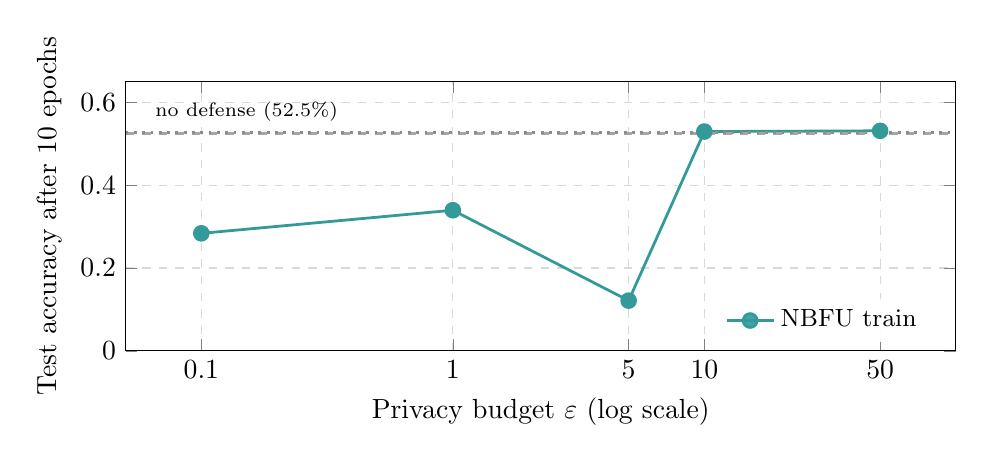
\begin{tikzpicture}
\begin{axis}[
    width=\columnwidth,
    height=5cm,
    xlabel={Privacy budget $\varepsilon$ (log scale)},
    ylabel={Test accuracy after 10 epochs},
    xmode=log,
    log basis x=10,
    xmin=0.05, xmax=100,
    ymin=0, ymax=0.65,
    grid=major,
    grid style={dashed, gray!30},
    legend pos=south east,
    legend style={font=\small, draw=none, fill=white, fill opacity=0.9, text opacity=1},
    mark size=2.5pt,
    every axis plot/.append style={line width=1pt},
    xtick={0.1,1,5,10,50},
    xticklabels={0.1, 1, 5, 10, 50},
]
% NBFU eps sweep accuracy
\addplot[color=teal!80, mark=*] coordinates {
    (0.1, 0.2837)
    (1.0, 0.3395)
    (5.0, 0.1212)
    (10.0, 0.5295)
    (50.0, 0.5313)
};
\addlegendentry{NBFU train}

% No-defense baseline (horizontal line)
\draw[dashed, gray!70, line width=1pt] (axis cs:0.05,0.5251) -- (axis cs:100,0.5251);
\node[anchor=south west, font=\scriptsize] at (axis cs:0.06,0.53) {no defense (52.5\%)};

% Clip-only baseline (horizontal line)
\draw[dotted, gray!90, line width=1pt] (axis cs:0.05,0.5277) -- (axis cs:100,0.5277);
\end{axis}
\end{tikzpicture}

\caption{Privacy--utility trade-off under NBFU on ChestMNIST classification. Sharp cliff at $\varepsilon \approx 5$--$10$. Dashed line: no-defense baseline. Pure clipping ($\sigma{=}0$, dotted) preserves utility.}
\label{fig:utility}
\end{figure}

\paragraph{Reconciling defense and utility.}
Our headline defense result (Section~\ref{sec:nbfu}) used $\varepsilon{=}5$, which the utility analysis shows is incompatible with stable training. This tension has three resolutions in practice:
\begin{enumerate}
\itemsep0pt
    \item \textbf{Round-targeted defense.} Geminio attacks at a single FL round (the round in which the malicious model is sent). If the defender activates NBFU only at suspect rounds---for example, when the global model parameters change abnormally between rounds---the utility cost is amortized over those rounds and is negligible in benign settings.
    \item \textbf{Higher $\varepsilon$ with higher $C$.} The clipping bound $C$ controls the noise magnitude (since $\sigma \propto C$). Tuning $C$ down reduces the per-element noise variance but tightens clipping. We did not optimize $C$ jointly with $\varepsilon$ in this study; an adaptive scheme analogous to~\citet{dpsfl2024} could move the cliff.
    \item \textbf{Defense-only deployment.} If the federated training has already converged when an attack is detected (e.g., during a fine-tuning round), accuracy degradation in the immediate round is acceptable.
\end{enumerate}

\paragraph{Note on dimensionality.} The optimizer updates only the 148K-parameter classifier head, so the utility cliff in Table~\ref{tab:utility} reflects noise added across that 148K subspace---but in the FL setup the shared gradient covers the full 11.3M parameters (Section~\ref{sec:setup}). NBFU applied where the optimizer also updates the backbone would face proportionally more aggregate noise and a more pronounced utility cliff. Full-model utility under NBFU is left to future work.


\section{Discussion}

\paragraph{Why language-guided attacks are an EMNLP concern.}
Geminio's interface is natural language. The attacker's discrimination ability scales with VLM quality: better VLMs $\to$ sharper text-image alignment $\to$ stronger gradient amplification on query-matching samples. Improvements in language-vision pretraining therefore enlarge the attack surface for federated systems. NBFU's invariance to amplification (Equation~\ref{eq:snr}) is what makes it a stable defense as VLMs continue to scale.

\paragraph{Practical guidance.}
NBFU has two knobs that must be set jointly: the clipping bound $C$ and the privacy budget $\varepsilon$. Our experiments suggest setting $C$ approximately equal to the expected median per-update gradient norm at the target batch size, then choosing $\varepsilon$ to satisfy regulatory requirements. The defense effect is robust over a wide $\varepsilon$ range (Figure~\ref{fig:eps}); the bigger sensitivity is to $C$ and to batch size.

\paragraph{Auxiliary observation.}
On medical, all three reconstruction algorithms reach a similar clean-baseline ceiling at 24{,}000 iterations (mean F1 $\approx 0.67$ across seeds). This may suggest Geminio's gradient amplification, rather than the choice of GIA algorithm, sets a practical upper bound on reconstruction quality at this iteration budget. Systematic investigation is left to future work.


\section{Related Work}

\paragraph{Gradient inversion attacks.}
DLG~\citep{dlg2019} introduced gradient leakage as a privacy threat; iDLG~\citep{idlg2020} added analytic label recovery. \citet{ig2020} replaced Euclidean distance with cosine similarity and added total-variation regularization, scaling the attack to ImageNet. GradInversion~\citep{gradinversion2021} added BatchNorm-statistic and feature-space priors for batch reconstruction. These remain the workhorse algorithms used as the reconstruction step in active-server attacks.

\paragraph{Active-server attacks.}
Robbing the Fed~\citep{robbing2022} introduced architecture-modification attacks; Fishing~\citep{fishing2023} amplified target gradients via output-layer parameter scaling. Geminio~\citep{geminio2024} generalized targeting to natural-language queries via VLMs. Our work focuses on defenses against this last family.

\paragraph{DP defenses.}
Differential privacy in deep learning was formalized by~\citet{dpsgd2016}; \citet{differentialprivacy2014} provide a foundation. \citet{mcmahan2018learning} introduced \emph{client-level} DP for FL with adjacency at the level of whole clients; our per-update-aggregate notion is closer to the per-round protections analyzed by~\citet{zhang2021clipping}, who study convergence under per-update clipping in heterogeneous FL and provide guidance on threshold selection (we discuss their results in Section~\ref{sec:nbfu-mechanism}). \citet{dpsfl2024} propose adaptive clipping with sparse updates to reduce DP noise impact, and~\citet{dp_gia_eval2025} empirically corroborate that calibrated DP-SGD reduces gradient inversion success on large pretrained models---consistent with our findings, though their evaluation does not include language-guided active attacks.

\paragraph{Non-DP defenses.}
\citet{geminio2024} themselves test gradient pruning, additive noise, and FedAvg, and report these are inconsistent or insufficient; our results confirm this for pruning and noise. Beyond DP, recent non-DP defenses include SVDefense~\citep{svdefense2025}, which projects gradients onto a low-rank subspace to remove inversion-relevant directions, and the convolutional variational bottleneck of~\citet{cvb2023}, which adds client-side variational noise driven by the model rather than a privacy budget. These approaches are complementary: NBFU provides a formal DP guarantee at known utility cost, while SVDefense and variational-bottleneck defenses target the inversion attacker without claiming DP. A comparison study at matched empirical defense level is left to future work.

\paragraph{Robust VLMs.}
TeCoA~\citep{tecoa2023}, FARE~\citep{fare2024}, and SimCLIP~\citep{simclip2024} adversarially fine-tune CLIP's vision encoder against input perturbations. Our results (Section~\ref{sec:vlm}) show that the threat model mismatch with Geminio means robustness in this sense does not transfer to FL gradient privacy: it raises loss-ratio amplification on medical and raises end-to-end attack F1 on UAV.


\section{Conclusion}

We studied defenses against Geminio, a language-guided gradient inversion attack that uses VLMs to target valuable client data with natural-language queries. We showed that adversarially robust VLMs do not protect against this attack: they raise Geminio's gradient-amplification loss ratio by 57--61\% on medical data, and on UAV imagery three of six robust variants raise mean end-to-end attack F1 above vanilla CLIP (multi-seed). NBFU---per-update L2 clipping plus calibrated Gaussian noise, providing $(\varepsilon,\delta)$-DP at the per-update aggregate---substantially reduces the attack across three reconstruction algorithms, driving mean F1 to zero on UAV at $\varepsilon{=}5$ and cutting medical F1 by half. A $\sigma{=}0$ ablation reveals that clipping and noise defend through complementary mechanisms: clipping disrupts scale-sensitive image priors, noise breaks scale-invariant cosine matching. The strongest defense regime ($\varepsilon{=}5$) destabilizes single-step training in our setup; we discuss round-targeted deployment as a path to reconcile defense and utility. As VLMs continue to scale, gradient-level DP appears more durable than encoder-level robustness as a privacy mechanism in federated learning, provided both clipping and noise are deployed together.


\section*{Limitations}

We highlight seven limitations.

First, we evaluate on a single architecture (ResNet-18). The SNR argument depends on $d$, the parameter count; very small models with $d \lesssim 10^5$ would have substantially higher SNR after defense and could be more reconstructable.

Second, our reconstruction quality metric, attack F1 at cosine threshold 0.90, is coarse at small batch sizes ($n{=}8$ admits only 9 discrete values). We report the continuous \emph{average} cosine similarity alongside F1 in Section~\ref{sec:nbfu-mechanism} to address metric variance, but a richer evaluation would include per-sample reconstruction quality histograms.

Third, we test three GIAs (DLG, IG, GradInversion) at full-layer scale and one (HF-GradInv) at all batch sizes; the former three exceed GPU memory at $n \ge 16$ in our setup. The batch-size sweep is therefore reported only for HF-GradInv.

Fourth, the SNR bound (Equation~\ref{eq:snr}) is an informal expectation argument, not a high-probability bound on the reconstruction error. A rigorous treatment would account for the directional structure of the reconstruction objective and the noise interaction with image priors.

Fifth, we evaluate the privacy--utility curve under NBFU on classifier-head training only (Section~\ref{sec:utility}); a full deployment that trains the backbone under NBFU may face larger utility costs due to the higher-dimensional clipping target.

Sixth, our DP guarantee is per-update aggregate $(\varepsilon,\delta)$ in the substitute-one-record neighboring relation, with sensitivity $2C$. Tighter record-level guarantees would require per-example clipping; presence/absence client-level DP would require sampling clients. We do not report cross-round composition; deployments must compose the per-round budget over training using a standard accountant.

Seventh, our attack coverage is restricted to gradient-matching GIAs (DLG, IG, GradInversion, HF-GradInv). More recent attacks leverage generative or denoising priors---e.g., GIFD~\citep{fang2023gifd} uses a pretrained GAN, and GUIDE~\citep{guide2025} uses a denoiser to clean reconstructed images---and may partially exploit image priors to overcome noisy gradients. We do not evaluate against these; doing so would require domain-specific pretrained generative models (no such models exist off-the-shelf for ChestMNIST X-rays or UAVScenes aerial imagery). Whether NBFU's defense margin holds against generative-prior attacks is left to future work, with the expectation that the $\sigma{=}0$ ablation's mechanism analysis still applies: noise breaks gradient-matching at the SNR level regardless of which prior the attacker uses.


\section*{Ethical Considerations}

This paper studies attacks and defenses in federated learning. Our defense, NBFU, is a constructive contribution: it provides a deployable mitigation for an existing published attack~\citep{geminio2024}. We make available no new attack capabilities beyond reproducing baselines from the literature for evaluation purposes. Our evaluation uses public benchmarks (ChestMNIST, UAVScenes); no private user data is collected or distributed.

A subtle ethical concern is our negative result on robust VLMs. We disclose this finding to prevent misallocation of defense engineering effort: practitioners should not assume that adversarially robust encoders, designed for a different threat model, transfer protection to federated gradient privacy. The mechanism we identify (Section~\ref{sec:vlm}) suggests this is a structural property, not an artifact of specific encoder weights.


\bibliography{custom}

\end{document}
